%package list
\documentclass{article}
\usepackage[top=3cm, bottom=3cm, outer=3cm, inner=3cm]{geometry}
\usepackage{graphicx}
\usepackage{url}
%\usepackage{cite}
\usepackage{hyperref}
\usepackage{array}
\usepackage{multicol}
\newcolumntype{x}[1]{>{\centering\arraybackslash\hspace{0pt}}p{#1}}
\usepackage{natbib}
\usepackage{pdfpages}
\usepackage{multirow}
\usepackage{float}
\usepackage[normalem]{ulem}
\useunder{\uline}{\ul}{}
\usepackage{svg}
\usepackage{amsmath}  
\usepackage{hyperref}
  
%%%%%%%%%%%%%%%%%%%%%%%%%%%%%%%%%%%%%%%%%%%%%%%%%%%%%%%%%%%%%%%%%%%%%%%%%%%%
%%%%%%%%%%%%%%%%%%%%%%%%%%%%%%%%%%%%%%%%%%%%%%%%%%%%%%%%%%%%%%%%%%%%%%%%%%%%
\newcommand{\csemail}{vmachacaa@unsa.edu.pe}
\newcommand{\csdocente}{Vicente Machaca Arceda}
\newcommand{\cscurso}{Algoritmos y Estructura de Datos}
\newcommand{\csuniversidad}{Universidad Nacional de San Agustín}
\newcommand{\csescuela}{Maestría en Ciencia de la Computación}
\newcommand{\cspracnr}{02}
\newcommand{\cstema}{Estructura de datos}
%%%%%%%%%%%%%%%%%%%%%%%%%%%%%%%%%%%%%%%%%%%%%%%%%%%%%%%%%%%%%%%%%%%%%%%%%%%%
%%%%%%%%%%%%%%%%%%%%%%%%%%%%%%%%%%%%%%%%%%%%%%%%%%%%%%%%%%%%%%%%%%%%%%%%%%%%


\usepackage[english,spanish]{babel}
\usepackage[utf8]{inputenc}
\AtBeginDocument{\selectlanguage{spanish}}
\renewcommand{\figurename}{Figura}
\renewcommand{\refname}{Referencias}
\renewcommand{\tablename}{Tabla} %esto no funciona cuando se usa babel
\AtBeginDocument{%
	\renewcommand\tablename{Tabla}
}

\usepackage{fancyhdr}
\pagestyle{fancy}
\fancyhf{}
\setlength{\headheight}{30pt}
\renewcommand{\headrulewidth}{1pt}
\renewcommand{\footrulewidth}{1pt}
\fancyhead[L]{\raisebox{-0.2\height}{
\includegraphics[width=3cm]{img/logo_unsa}}}
\fancyhead[C]{}
\fancyhead[R]{\fontsize{7}{7}\selectfont	\csuniversidad \\ \csescuela \\ \textbf{\cscurso} }
\fancyfoot[L]{MSc. Vicente Machaca}
\fancyfoot[C]{\cscurso}
\fancyfoot[R]{Página \thepage}


\begin{document}
	
	\vspace*{10px}
	
	\begin{center}	
		\fontsize{17}{17} \textbf{ Práctica \cspracnr}
	\end{center}
	%\centerline{\textbf{\underline{\Large Título: Informe de revisión del estado del arte}}}
	%\vspace*{0.5cm}
	

	\begin{table}[h]
		\begin{tabular}{|x{4.7cm}|x{4.8cm}|x{4.8cm}|}
			\hline
			\textbf{DOCENTE} & \textbf{CARRERA}  & \textbf{CURSO}   \\
			\hline
			\csdocente & \csescuela & \cscurso    \\
			\hline
		\end{tabular}
	\end{table}	
	
	
	\begin{table}[h]
		\begin{tabular}{|x{4.7cm}|x{4.8cm}|x{4.8cm}|}
			\hline
			\textbf{PRÁCTICA} & \textbf{TEMA}  & \textbf{DURACIÓN}   \\
			\hline
			\cspracnr & \cstema & --   \\
			\hline
		\end{tabular}
	\end{table}
	
	\section{Datos de los integrantes}
        	\begin{itemize}
        		\item Grupo: \textbf{\large{2}}
        		\item Integrantes:
        		\begin{itemize}
        			\item EDER ALONSO AMPUERO ATAMARI
        			\item HOWARD FERNANDO ARANZAMENDI MORALES
                    \item JOSE EDISON PEREZ MAMANI
                    \item HENRRY IVAN ARIAS MAMANI
        		\end{itemize}		
        	\end{itemize}
    \section{Repositorio de GITHUB}
           Url Github: \href{https://github.com/hAriasm/Practica2_ayed}{Práctica 2}
	\section{Estructuras de Datos}
        \subsection{BTree}
            \paragraph{}
   zzzzzzzzzz


        \subsection{AVL}

        El árbol AVL recibe su nombre de las iniciales  de sus inventores, Georgii Adelson-Velskii y Yevgeniy Landis. Dieron a conocer esto mediante la publicación de un artículo en 1962, "Un algoritmo para organizar la información" ("Un algoritmo para organizar la información").
        
        Un árbol AVL es un árbol de búsqueda binaria que tiene una altura equilibrada: para cada nodo x, las alturas de los subárboles izquierdo y derecho de x difieren en 1 como máximo. Para implementar un árbol AVL, mantenemos un atributo adicional en cada nodo: x.h es la altura del nodo x. Como para cualquier otro árbol binario de búsqueda T, asumimos que T.root apunta al nodo raíz.
        
        El árbol AVL siempre está equilibrado de  modo que para todos los nodos, la altura de la rama izquierda no difiera en más de una unidad de la altura de la rama derecha o viceversa. Gracias a esta forma de equilibrio, la complejidad de una búsqueda en uno de estos árboles se mantiene siempre en el orden de complejidad O(log n). El factor de equilibrio puede almacenarse directamente en cada nodo o calcularse a partir de la altura de los subárboles.
        
        Para lograr este equilibrio, la inserción y eliminación de  nodos debe realizarse de manera especial. Si la condición de equilibrio se rompe al realizar una operación de inserción o eliminación, se debe realizar una serie de rotaciones de  nodos.
         
         \subsubsection{Resultados del experimento}
         \begin{itemize}
            \item En la figura \ref{fig:avlBusqueda} mostramos la búsqueda del nodo 22 con resultado de no encontrado
           \item En la figura \ref{fig:avlBusqueda} mostramos nuestro árbol inicial con 11 nodos.
           \item En la figura \ref{fig:avlBusqueda} mostramos nuestro árbol inicial con 11 nodos.

           \item En la figura \ref{fig:avlInicial} mostramos nuestro árbol inicial con 11 nodos.
           \item En la figura \ref{fig:avlIsertion} mostramos el árbol luego de insertar un nodo nuevo.
           \item En la figura \ref{fig:avldelete} mostramos luego de eliminar un nodo.
           \item En la figura \ref{fig:avldelete2} mostramos luego de eliminar el nodo raíz.
         \end{itemize}
         \begin{figure}[htbp]
              \centering
              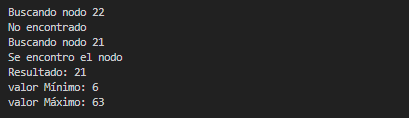
\includegraphics[width=\textwidth]{img/busquedaAVL.png}
              \caption{Árbol AVL búsqueda variada}
              \label{fig:avlBusqueda}
            \end{figure}
            \begin{figure}[htbp]
              \centering
              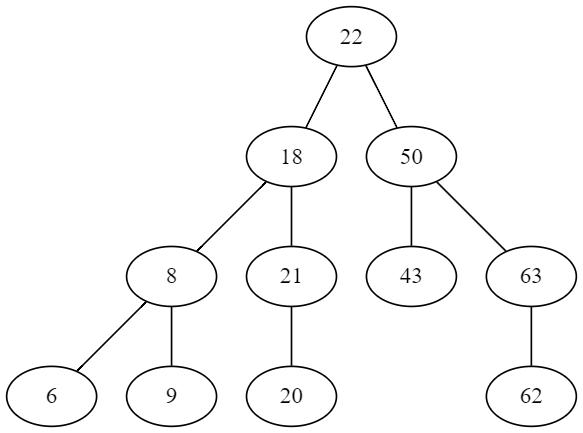
\includegraphics[width=0.5\textwidth]{img/avltree.png}
              \caption{Árbol AVL inicial}
              \label{fig:avlInicial}
            \end{figure}
            \begin{figure}[htbp]
              \centering
              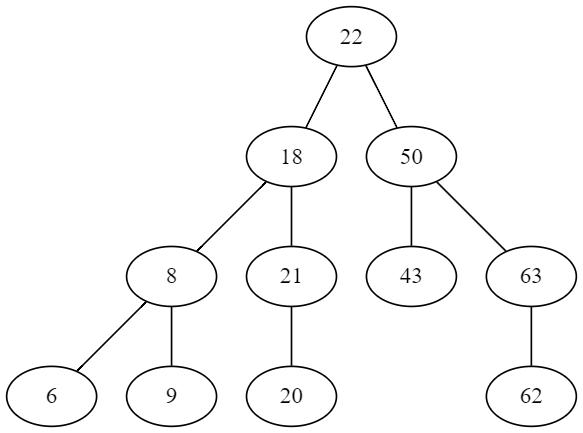
\includegraphics[width=0.5\textwidth]{img/avltree.png}
              \caption{Árbol AVL inicial}
              \label{fig:avlInicial}
            \end{figure}
            \begin{figure}[htbp]
              \centering
              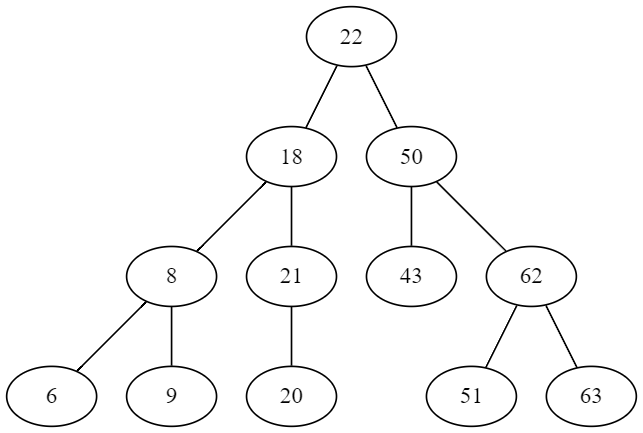
\includegraphics[width=0.5\textwidth]{img/avltree-insertion.png}
              \caption{Árbol AVL con inserción }
                \label{fig:avlIsertion}
            \end{figure}
            \begin{figure}[htbp]
              \centering
              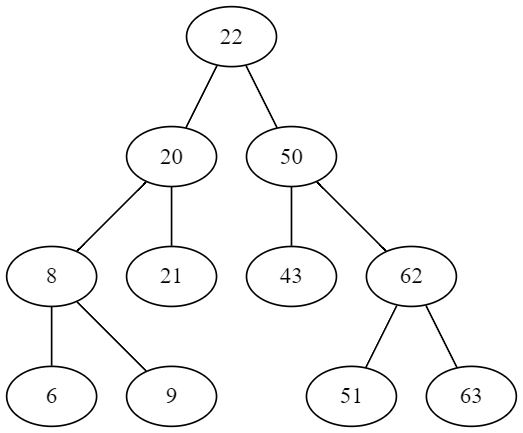
\includegraphics[width=0.5\textwidth]{img/avltree-deletion.png}
              \caption{Árbol AVL con eliminación nodo}
            \label{fig:avldelete}
            \end{figure}
             \begin{figure}[htbp]
              \centering
              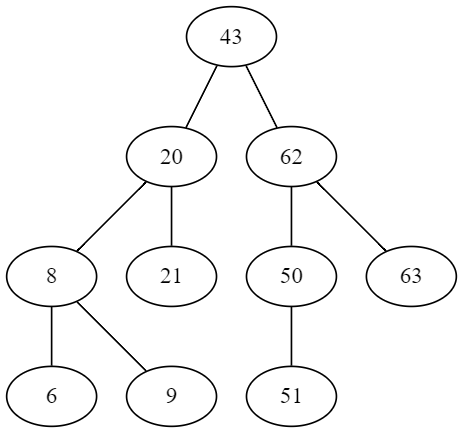
\includegraphics[width=0.5\textwidth]{img/avltree-deletion-2.png}
              \caption{Árbol AVL con eliminación de la raíz}
              \label{fig:avldelete2}
            \end{figure}

    \section{Conclusiones}
        \begin{itemize}
                 \item  ssss
                 \item	ssss
                 \item Un árbol AVL se mantiene ordenado, pero hay mas rotaciones en las inserciones que en las eliminaciones, su costo para buscar, eliminar, insertar  es de O(Log n).
                 \item  
        \end{itemize}

    \section{Referencias}
  \begin{enumerate}
    \item 1
    \item 1
    \item 1
    \item 1
    \item 1
    \item 1
    \item 1
    \item 1
    \item 1
    \item 1
  \end{enumerate}

\end{document} 